\documentclass[11pt]{article}
\usepackage{amsfonts}
\usepackage{hyperref}
\usepackage{graphicx,subfigure}
\usepackage{epsfig}
\usepackage{hyperref}
\usepackage{amsmath}
\usepackage{amssymb}
\usepackage{algorithm}
\usepackage{algorithmic}
\usepackage{url}
\usepackage{enumerate}
\usepackage{amsfonts}
\usepackage{boxedminipage}
\usepackage{xcolor}
 \usepackage{framed}

\usepackage{tcolorbox}

\usepackage{rotating}
\usepackage{soul}
\usepackage{mathtools}

\usepackage{array}
\usepackage{multirow}
\usepackage{color}
\usepackage{tikz}


\usepackage{mathabx}
\usepackage{tabularx,ragged2e,booktabs,caption}
\usepackage{enumitem}

\usepackage{cancel}
\usepackage{ulem,lipsum}
\usepackage{dsfont}

\newcommand{\overbar}[1]{\mkern 1.5mu\overline{\mkern-1.5mu#1\mkern-1.5mu}\mkern 1.5mu}

\oddsidemargin=0.15in
\evensidemargin=0.15in
\topmargin=-.5in
\textheight=9in
\textwidth=6.25in

\DeclarePairedDelimiter{\floor}{\lfloor}{\rfloor}
\DeclarePairedDelimiter{\ceil}{\lceil}{\rceil}
\DeclareGraphicsExtensions{.gif, .ps, .eps, .png}
\DeclareGraphicsRule{.gif}{png}{}{`convert #1 'png:-'}

\DeclareGraphicsExtensions{.gif, .ps, .eps, .png}
\DeclareGraphicsRule{.gif}{png}{}{`convert #1 'png:-'}

\newcommand{\inprod}[2]{\left\langle #1,#2\right\rangle}
\newcommand{\norm}[1]{\left\| #1\right\|}
\newcommand{\pmat}[1]{\begin{pmatrix} #1\end{pmatrix}}
\newcommand{\cB}{\mathcal{B}}
\newcommand{\bN}{\mathbb{N}\,}

\newcommand*{\vertbar}{\rule[-1ex]{0.5pt}{2.5ex}}
\newcommand*{\horzbar}{\rule[.5ex]{2.5ex}{0.5pt}}

\newcommand{\R}{\ensuremath{\mathbb{R}}}
 % \newcommand{\E}{\ensuremath{\mathbb{E}}}
 \newcommand{\N}{\ensuremath{\mathbb{N}}}
 %newcommand{\C}{\ensuremath{\mathbb{C}}}
 \newcommand{\Tr}{\ensuremath{\top}}
 \newcommand{\Prob}{\ensuremath{\mathbb{P}}}
 \newcommand{\Nc}{\mathcal{N}}
  \newcommand{\Ac}{\mathcal{A}}
  \newcommand{\Dc}{\mathcal{D}}

 % IML
 % ----
 \newcommand{\Xc}{\mathcal{X}}
 \newcommand{\Yc}{\mathcal{Y}}
 \newcommand{\Hc}{\mathcal{H}}
\newcommand{\innerr}[2]{{\left\langle #1\,,\,#2 \right\rangle}}

 % ---

%\newcommand{\norm}[1]{\left|\left| #1 \right|\right|}


\newcommand{\plim}{\stackrel{p}{\rightarrow}}
\newcommand{\aslim}{\stackrel{a.s.}{\rightarrow}}
\newcommand{\dlim}{\stackrel{d}{\rightarrow}}

% distributed as
\newcommand{\iid}{\stackrel{\text{iid}}{\sim}}
\newcommand{\ind}{\stackrel{\text{ind.}}{\sim}}
\newcommand{\indep}{\stackrel{\text{indep.}}{\sim}}
\newcommand{\V}[1]{\mathbf{#1}}
\newcommand{\Vhat}[1]{\ensuremath{\hat{\mathbf{#1}}}}

\title{{\large{Introduction to Machine Learning (67577) \\
\vphantom{} Model Selection and Evaluation }}}

\date{Special Covid-19 edition, 4/2020}

\usepackage{graphicx,subfigure}
% As of 2010, we use the hyperref package to produce hyperlinks in the
% resulting PDF.  If this breaks your system, please commend out the
% following usepackage line and replace \usepackage{icml2011} with
% \usepackage[nohyperref]{icml2011} above.
\usepackage{hyperref}

% \usepackage{icml2011}

\usepackage{amsmath}
\usepackage{amssymb}

\usepackage{algorithm}
\usepackage{algorithmic}
\algsetup{indent=2em}


%% \usepackage{rotating}
%% \usepackage{array}
%% \usepackage{multirow}
%% \usepackage{color}

%% \usepackage{tikz}

\usepackage{url}

\newtheorem{definition}{Definition}
\newtheorem{lemma}{Lemma}
\newtheorem{corollary}{Corollary}
\newtheorem{theorem}{Theorem}
\newtheorem{proposition}{Proposition}
\newtheorem{assumption}{Assumption}
\newtheorem{example}{Example}
\newtheorem{remark}{Remark}
\newtheorem{claim}{Claim}
\newtheorem{exercise}{Exercise}
\newtheorem{discussion}{Discussion}


\newcommand{\gb}[1]{{\boldsymbol{#1}}}
\newcommand{\valpha}{\gb{\alpha}}
\newcommand{\vmu}{\gb{\mu}}
\newcommand{\vnu}{\gb{\nu}}
\newcommand{\vxi}{\gb{\xi}}
\newcommand{\vtheta}{\gb{\theta}}
\newcommand{\vrho}{\gb{\rho}}
\newcommand{\vbeta}{\gb{\beta}}
\newcommand{\vtau}{\gb{\tau}}
\newcommand{\vbalpha}{\gb{\alpha^\star}}
\newcommand{\vbbeta}{\gb{\beta^\star}}
\newcommand{\vtalpha}{\gb{\tilde{\alpha}}}
\newcommand{\vlambda}{\gb{\lambda}}
\newcommand{\slambda}{\bar{\vlambda}}
\newcommand{\stheta}{\bar{\vtheta}}
\newcommand{\vphi}{\gb{\phi}}
\newcommand{\vsigma}{\gb{\sigma}}

\newcommand{\x}{{\mathbf x}}
\newcommand{\y}{{\mathbf y}}
\newcommand{\z}{{\mathbf z}}
\newcommand{\w}{{\mathbf w}}
\newcommand{\bw}{\bar{\w}}
\newcommand{\bF}{\bar{F}}
\renewcommand{\v}{{\mathbf v}}
\renewcommand{\u}{{\mathbf u}}
\newcommand{\e}{{\mathbf e}}
\newcommand{\bsig}{{\mathbf \sigma}}
\newcommand{\rE}{{\mathbf E}}
\newcommand{\sgn}{{\mathrm{sgn}}}
\newcommand{\cF}{{\cal F}}
\newcommand{\pr}{\mathbb{P}}
\newcommand{\rV}{{\mathrm {Var}}}
\newcommand{\tr}{{\mathrm{tr}}}
\newcommand{\trans}{\dagger}
\newcommand{\diag}{{\mathrm{diag}}}
\newcommand{\lspan}{{\mathrm{span}}}
\renewcommand{\r}{{\mathbf{r}}}
\newcommand{\tL}{\tilde{L}}
\newcommand{\hL}{\hat{L}}

\newcommand{\cD}{\mathcal{D}}
\newcommand{\bE}{\mathbb{E}\,}


\newcommand{\BlackBox}{\rule{1.5ex}{1.5ex}}
\newenvironment{proof}{\par\noindent{\bf Proof\ }}{\hfill\BlackBox\\[2mm]}

\newcommand{\reals}{\mathbb{R}}
\newcommand{\Y}{\mathcal{Y}}
\newcommand{\X}{\mathcal{X}}
\renewcommand{\H}{\mathcal{H}}
\newcommand{\E}{\mathbb{E}}
\newcommand{\D}{\mathcal{D}}
\newcommand{\V}{\mathcal{V}}
%\newcommand{\U}{\mathcal{U}}
\newcommand{\F}{\mathcal{F}}
\newcommand{\inner}[1]{\langle #1 \rangle}
\newcommand{\half}{\frac{1}{2}}
\newcommand{\thalf}{\tfrac{1}{2}}
\newcommand{\eqdef}{\stackrel{\mathrm{def}}{=}}
\newcommand{\err}{\mathrm{err}}
\newcommand{\opt}{\mathrm{opt}}
\newcommand{\herr}{\widehat{\err}}
\newcommand{\hopt}{\hat{\opt}}
\newcommand{\eopt}{\epsilon_{\mathrm{opt}}}
\newcommand{\eapp}{\epsilon_{\mathrm{app}}}
\newcommand{\eest}{\epsilon_{\mathrm{est}}}
\newcommand{\halg}{\tilde{h}}
\newcommand{\empf}{\hat{F}_{\lambda}}
\newcommand{\T}{\mathrm{time}}
\newcommand{\erf}{\mathrm{erf}}
\newcommand{\sig}{\mathrm{sig}}
\newcommand{\poly}{\mathrm{poly}}

\newcommand{\rank}{\mathrm{rank}}
\newcommand{\supp}{\mathrm{supp}}
\newcommand{\spn}{\mathrm{span}}
\newcommand{\image}{\mathrm{image}}


\DeclareMathOperator*{\argmin}{argmin} % Declares argmin and ensures super and subscripts are located nicely above/below such as in \min
\DeclareMathOperator*{\argmax}{argmax} % Declares argmin and ensures super and subscripts are located nicely above/below such as in \min
\DeclareMathOperator*{\prob}{\mathbb{P}}

\renewcommand{\eqref}[1]{Equation~(\ref{#1})}
\newcommand{\figref}[1]{Figure~\ref{#1}}
\newcommand{\secref}[1]{Section~\ref{#1}}
\newcommand{\thmref}[1]{Theorem~\ref{#1}}
\newcommand{\lemref}[1]{Lemma~\ref{#1}}
\newcommand{\defref}[1]{Definition~\ref{#1}}
\newcommand{\corref}[1]{Corollary~\ref{#1}}

%\newcommand{\comment}[1]{\textcolor{red}{\textbf{#1}}}
\newcommand{\mathcomment}[1]{\color{red}{\textbf{#1}}}

\newcommand{\indct}[1]{\boldsymbol{1}\!\left[ #1 \right]}

\newcommand{\blambda}{\bar{\lambda}}
\newcommand{\bA}{\bar{A}}
\newcommand{\bI}{\bar{I}}

\newcommand{\vect}{\mathrm{vec}}


\newcommand{\coursename}{Introduction to Machine Learning (67577)}

\newcommand{\handout}[5]{
%   \renewcommand{\thepage}{#1-\arabic{page}}
   \noindent
   \begin{center}
   \framebox{
      \vbox{
    \hbox to 5.78in { {\bf \coursename}
         \hfill #2 }
       \vspace{4mm}
       \hbox to 5.78in { {\Large \hfill #5  \hfill} }
       \vspace{2mm}
       \hbox to 5.78in { {\it #3 \hfill #4} }
      }
   }
   \end{center}
   \vspace*{4mm}
}

\newcommand{\notes}[5]{
%   \renewcommand{\thepage}{#1-\arabic{page}}
   \noindent
   \begin{center}
    \hbox to 5.78in { {\bf \coursename}  \hfill #2}
       \vspace{14mm}
       \hbox to 5.78in { {\Large \hfill #5  \hfill} }
   \end{center}
   \vspace*{4mm}
}

% Lecture notes:
\newcommand{\lecture}[5]{\handout{#1}{#3}{Lecturer:
#4}{Scribe: #5}{Lecture #1: #2}}

\newcommand{\recitation}[5]{\handout{#1}{#3}{#4}{ #5}{Recitation #1: #2}}

% Exam:
\newcommand{\exam}[1]{\handout{#1}{}{}{}{Exam}}
\newcommand{\homeexam}[2]{\handout{#1}{}{}{Due:
#2}{Home Exam}}
\newcommand{\examanswer}[1]{\handout{X}{}{by: #1}{}{Exam - Answers}}

% New exercise
\newcommand{\problemset}[2]{\handout{#1}{}{}{Due:
#2}{Problem Set #1}}

% School solution
\newcommand{\solution}[2]{\handout{#1}{}{}{Written by: #2}{Problem Set #1 - Solution}}

% Submitted solution
\newcommand{\exanswer}[2]{\handout{#1}{}{by: #2}{}{Problem Set #1 - Answers}}

\begin{document}
\maketitle

\tableofcontents
\pagebreak

Suggested Reading:
\begin{itemize}
  \item Model selection and model evaluation: ESL 7.2
  \item Bias-Variance Tradeoff and Decomposition: UML 5.2, ESL 7.3
  \item k-Fold Cross Validation: ESL 7.10
  \item The ``snooping mistake'' in Cross Validation for model evaluation: ESL 7.10.2
  \item Bootstrap for model evaluation: ESL 7.11
  \item Feature selection
\end{itemize}


\section{Introduction}

\subsection{Model Selection}

So far in this course we've seen learning algorithms (for classification and
regression) and meta-algorithms that can be applied on top of an existing
learning algorithm. The next step in our expertise is to be able to know 
\begin{itemize}
  \item Which of the algorithms we have at our disposal to use on a certain
    problem?
  \item How to choose the tuning parameters?
\end{itemize}
~\\
This is called {\bf Model Selection.} 
\\~\\
What do we mean by the term ``tuning parameters''?
As we've seen, ``choosing an algorithm'' typically means choosing a {\bf family} of
learning algorithms, namely a collection of learning algorithms indexed by one
or more parameters. We can call these tuning parameters. 
Some examples we've seen:
\begin{itemize}
  \item choosing $k$ in $k$-Nearest Neighbors
  \item choosing the regularization parameter $\lambda$ in soft-SVM
  \item choosing the regularization parameter $\lambda$ in Lasso, Ridge Regression or
    $\ell_1$-regularized logistic regression
  \item choosing the maximal tree depth and pruning regularization parameter in
    CART classification / regression trees
\end{itemize}
~\\
Also if we've using a meta-algorithm such as bagging or boosting, we'll need to
choose any tuning parameters of the base learning {\bf and also} to choose the number
of bagging / boostrap iteration $B$. If we're using de-correlation in bagging,
there might be tuning parameters associated with that (e.g. the number $k$ of
allowed coordinates for a split in Random Forest).
\\~\\
So model selection is the choice of model and any tuning parameters. When 
we are
finished with our model selection, we have a completely specified learning algorithm
that we can train on our training sample, and use for prediction on new samples.

\subsection{Model Evaluation}

Another next step in our expertise is to be able to estimate the performance
(generalization error) of the model we've chosen - before we actually go ahead
and use it on
new samples. This is important for a number
of reasons:
\begin{itemize}
  \item One, if our estimate for the generalization error of our selected
model is poor, we may be working with the wrong
learning algorithm for this problem - maybe it would be best to go back to the
model selection stage and come up with new candidates. 
\item Two, very often when
using machine learning to solve real problems, we'll
want to know how our chosen learner will perform before we actually start using it.
(For example, think about a credit model learning system predicting which
customers will default on their loans.)
\end{itemize}

\subsection{What is the generalization error, exactly?}



Assume we have a loss function $\ell(\cdot,\cdot)$. 
The {\bf empirical risk} of an hypothesis $h:\X\to\Y$ 
is always defined simply by 
\[
L_S(h) = \sum_{i=1}^m \ell(h(x_i),y_i))
\]
where $S=\left\{ (x_i,y_i \right\}_{i=1}^m$ is our training sample.
\\~\\
However, our definition of {\bf generalization error} 
 depends on our data-generation model.
We've actually seen several definitions of {\bf generalization error} 
in this course already:

\begin{itemize}
  \item {\bf No data-generation model.}
    If we don't assume anything about how data is generated, the only definition
    of generalization error is on a new test set, unseen by the learner during
    training. If we have such a test set 
    $T=\left\{ (x_j,y_j) \right\}_{j=1}^{|T|}$
      then the generalization error of a chosen hypothesis $h$ is simply the average 
        \[
        L(h) = \sum_{j=1}^{|T|} \ell(h(x_j),y_j))
\]
\item {\bf Probability distribution on $\X$, and unknown labeling function
  $f:\X\to\Y$}
    If make the same assumption as the PAC model, the generalization error is 
 \[
   L_{\Dc,f}(h) = \E_{x\sim\Dc} [\ell(h(x),f(x)]
\]
\item {\bf Probability distribution on $\X\times \Y$}
    If make the same assumption as the Agnostic PAC model, the generalization error is 
 \[
   L_{\Dc}(h) = \E_{(x,y)\sim\Dc} [\ell(h(x),y]
\]
      
\end{itemize}
~\\
Just be mindful and pay attention about the actual definition being used in
different cases.



\section{Bias-Variance}

It's crucial to understand the behavior of generalization error as we make our
hypothesis $\Hc$ smaller or larger, and as we change the learning algorithm
$\Ac$ that chooses $h_S\in\Hc$. 


\subsection{Bias-Variance decomposition for square error loss}

In a regression problem, when using the square error loss, the generalization
error can be written as the sum of the variance and the square of the bias. 
\\~\\
Assume we have a training set $S={(x_i,y_i)}$. 
       We obtain a test set $T=(\tilde{x}_j,\tilde{y}_j)$. 
       We form the response vector of the test set,
       $\tilde{\V{y}}=(\tilde{y}_1,\ldots,\tilde{y}_{|T|})$.
      We use a learning algorithm trained on $S$ to obtain $h_S$, 
      and write $\hat{\tilde{y_j}}=h_S(\tilde{x}_j)$  for the predictions
      of $h_S$ on the test set $T$. We have a vector $\hat{\tilde{\V{y}}}$ of
      predictions. If we use the square error loss, then the 
      generalization error (as measured  on the test $T$) is simply
    $\norm{\hat{\tilde{\V{y}}}-\tilde{\V{y}}}^2$. 
      Now, since the training sample $S$ is a random set, $h_S$ is a random
      hypothesis, and
      therefore $\hat{\tilde{\V{y}}}$ is a random vector - all with respect to
      the random choice of $S$. 
      Let us  write $\mathbb{E}$ for the expectation with respect to the random
      choice of $S$. (This could be a random choice of $x_1,\ldots x_m$, or
    a random choice of $(x_1,y_1),\ldots,(x_m,y_m)$, for example.) 
\\~\\
      We have:


       \begin{eqnarray*}
         \E \norm{\tilde{\V{y}}-\hat{\tilde{\V{y}}}}^2 &=& 
         \E \norm{\tilde{\V{y}}-\E\hat{\tilde{\V{y}}} + \E \hat{\tilde{\V{y}}} -
         \hat{\tilde{\V{y}}}}^2 \\
         &=&  
         \E \norm{\tilde{\V{y}}-\E\hat{\tilde{\V{y}}} }^2
         +
         \E \norm{ \E \hat{\tilde{\V{y}}} -
         \hat{\tilde{\V{y}}}}^2
         + 2 \E \innerr{ 
           \tilde{\V{y}}-\E\hat{\tilde{\V{y}}} 
         }
         {
           \E \hat{\tilde{\V{y}}} -
         \hat{\tilde{\V{y}}}
         }\\
&=& 
    \norm{\tilde{\V{y}}-\E\hat{\tilde{\V{y}}} }^2
         +
         \sum_{i=1}^m Var(\hat{\tilde{y}}_i)
       \end{eqnarray*}


       What did we find?
       \begin{itemize}
         \item The term $\norm{\tilde{\V{y}}-\E\hat{\tilde{\V{y}}} }$ is the
           {\bf bias} of the learner we used. It quantifies the distance between
           the typical prediction $\E\hat{\tilde{\V{y}}}$ (typical over the choice of
           training sample $S$) and the true label
           $\tilde{\V{y}}$.
         \item The term $\sum_{i=1}^m Var(\hat{\tilde{y}}_i)$ is the {\bf
           variance} of the learner we used. It quantities the variability in
           the predicted labels,  as a result of the randomness in the training
           sample $S$.

       \end{itemize}

       So we have decomposed the generalization error - the performance of
       predicting new labels - into 
       the square of the bias, plus the variance.
\\~\\
       Here is an example you can do yourself in simulation - in polynomial
       fitting:


\begin{figure}[H]
  \centering
  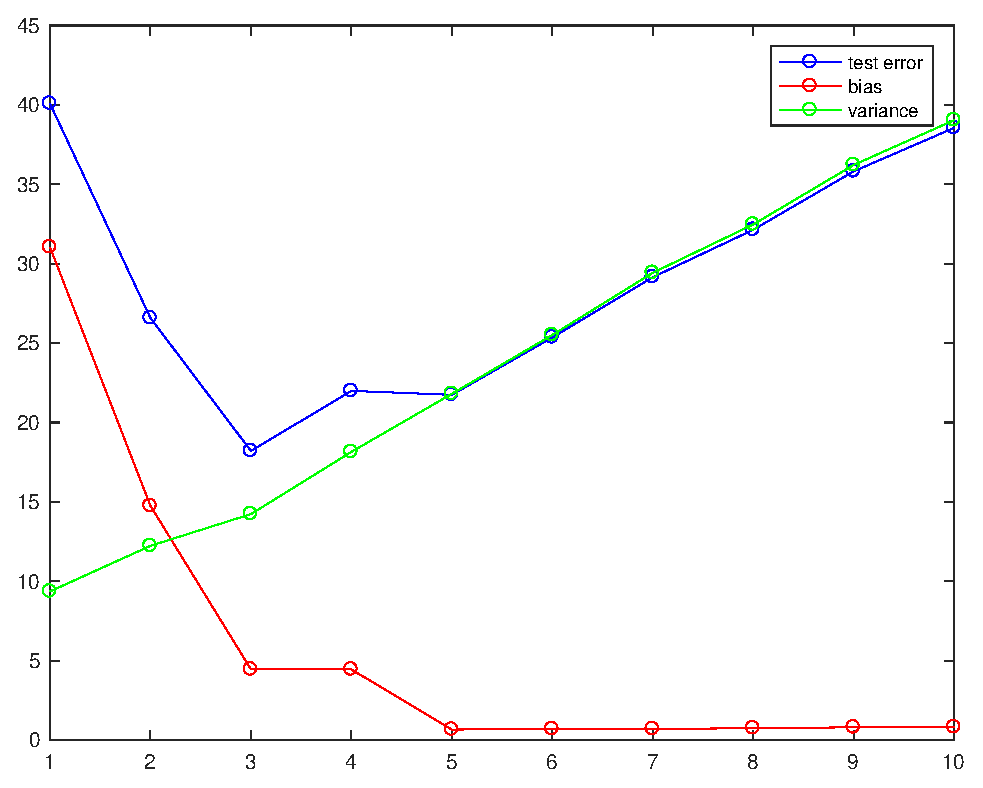
\includegraphics[width=3in]{poly_bias_variance.eps}
  \caption{Bias-Variance decomposition in polynomial fitting. Horizontal axis:
  fitted polynomial degree.}
\end{figure}

Here are two other examples of the bias-variance decomposition for square loss - 
\begin{figure}[H]
  \centering
  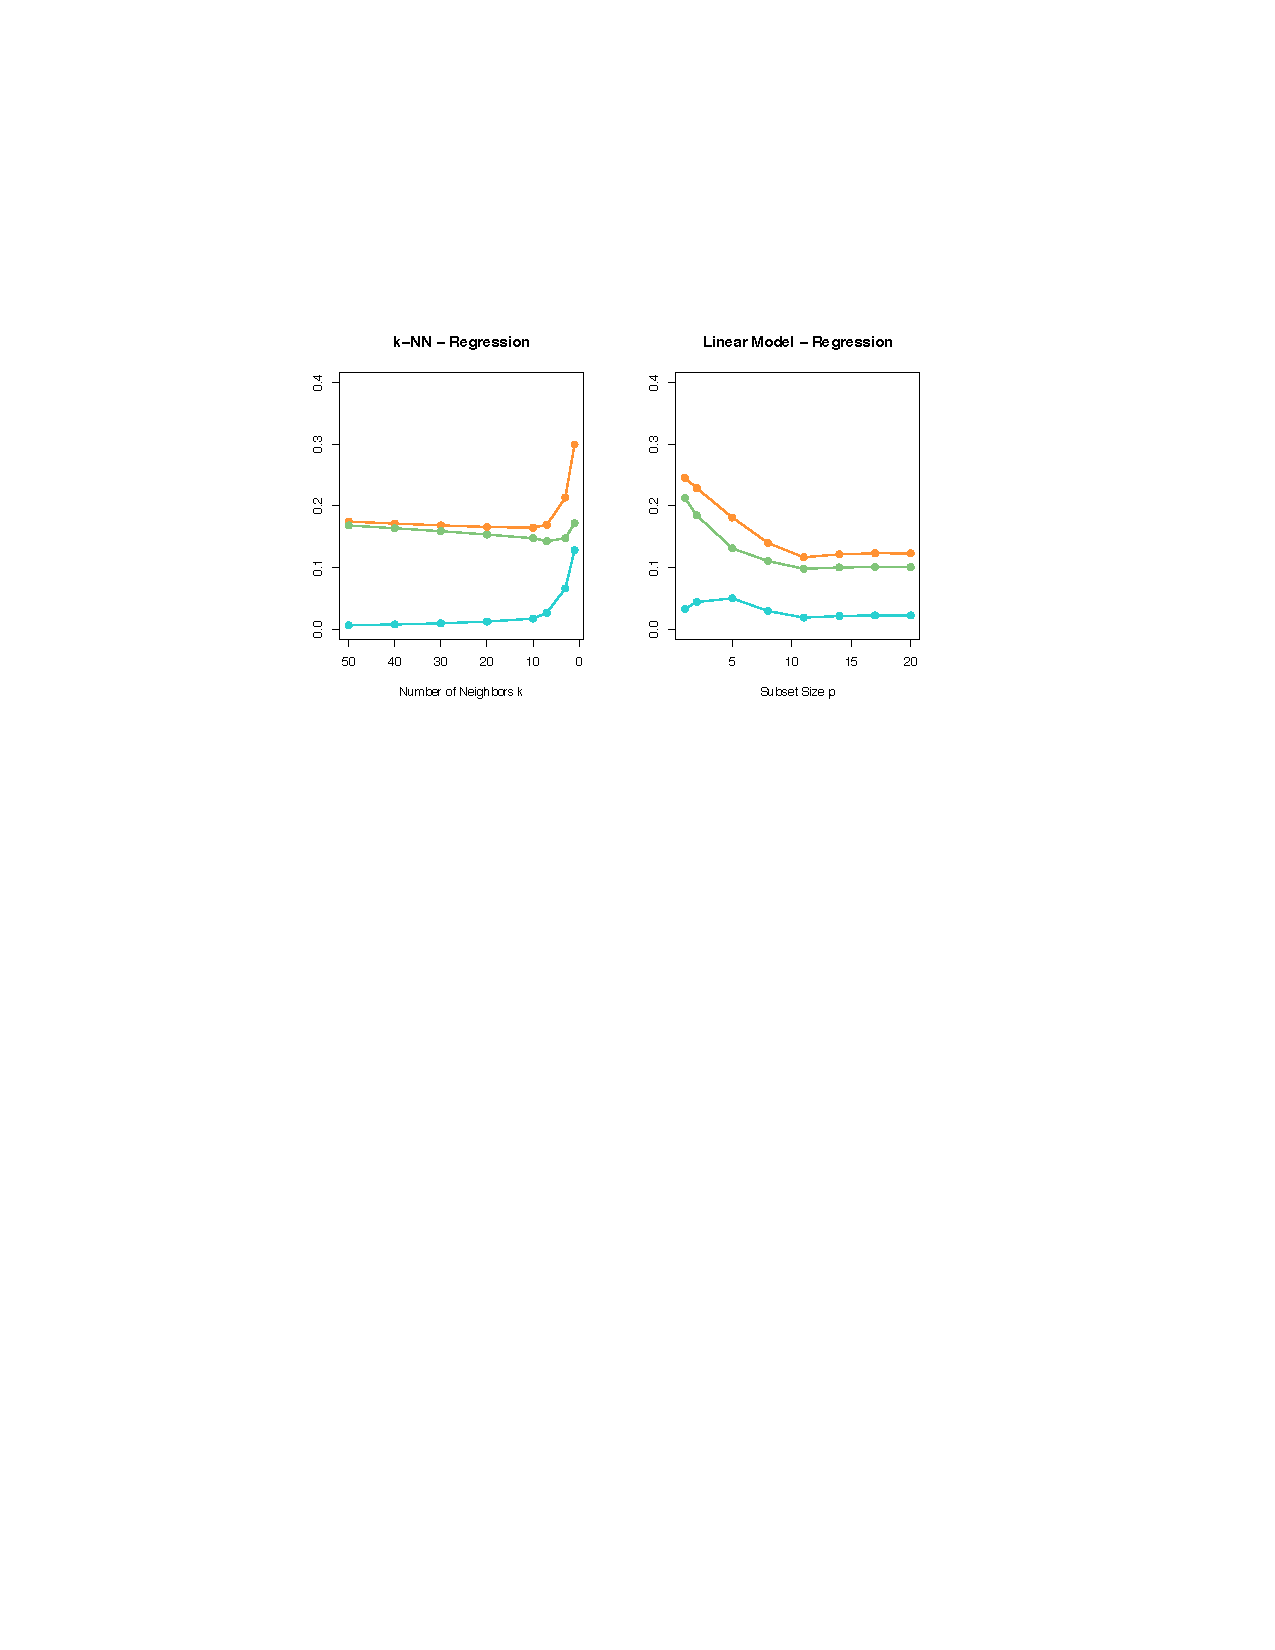
\includegraphics[width=5in]{esl_bias_variance_regression.pdf}
  \caption{Bias-Variance decomposition in simulation. Left: $k$-NN regression. Right:
    Best-subset regression. Horizontal axis - left: $k$ the number of nearest
    neighbors, right: $p$ the subset size. Orange - generalization error, green
    - square bias, blue - variance.
  Source: ESL}
\end{figure}


There are other bias-variance decompositions (see the textbooks). It is possible
to derive bias-variance decompositions for classifiers, but they are not so
elegant. 

%\subsection{The PAC view of bias-variance tradeoff}

\subsection{The bias-variance tradeoff}

Even when we don't have an elegant decomposition of the generalization error as
a sum of bias and variance, the {\bf bias-variance tradeoff}, which was 
mentioned every lecture so far in this course, is a general phenomenon. 
In any way we choose to measure the complexity of the hypothesis class $\Hc$
(VC-dimension, degree of polynomial, linear dimension of linear model, maximal
  decision tree
depth, etc \ldots) 
or
the learner $\Ac$  (regularization parameter, $k$ in $k$-NN, etc) we always
observe a tradeoff of this form:

\begin{figure}[H]
  \centering
  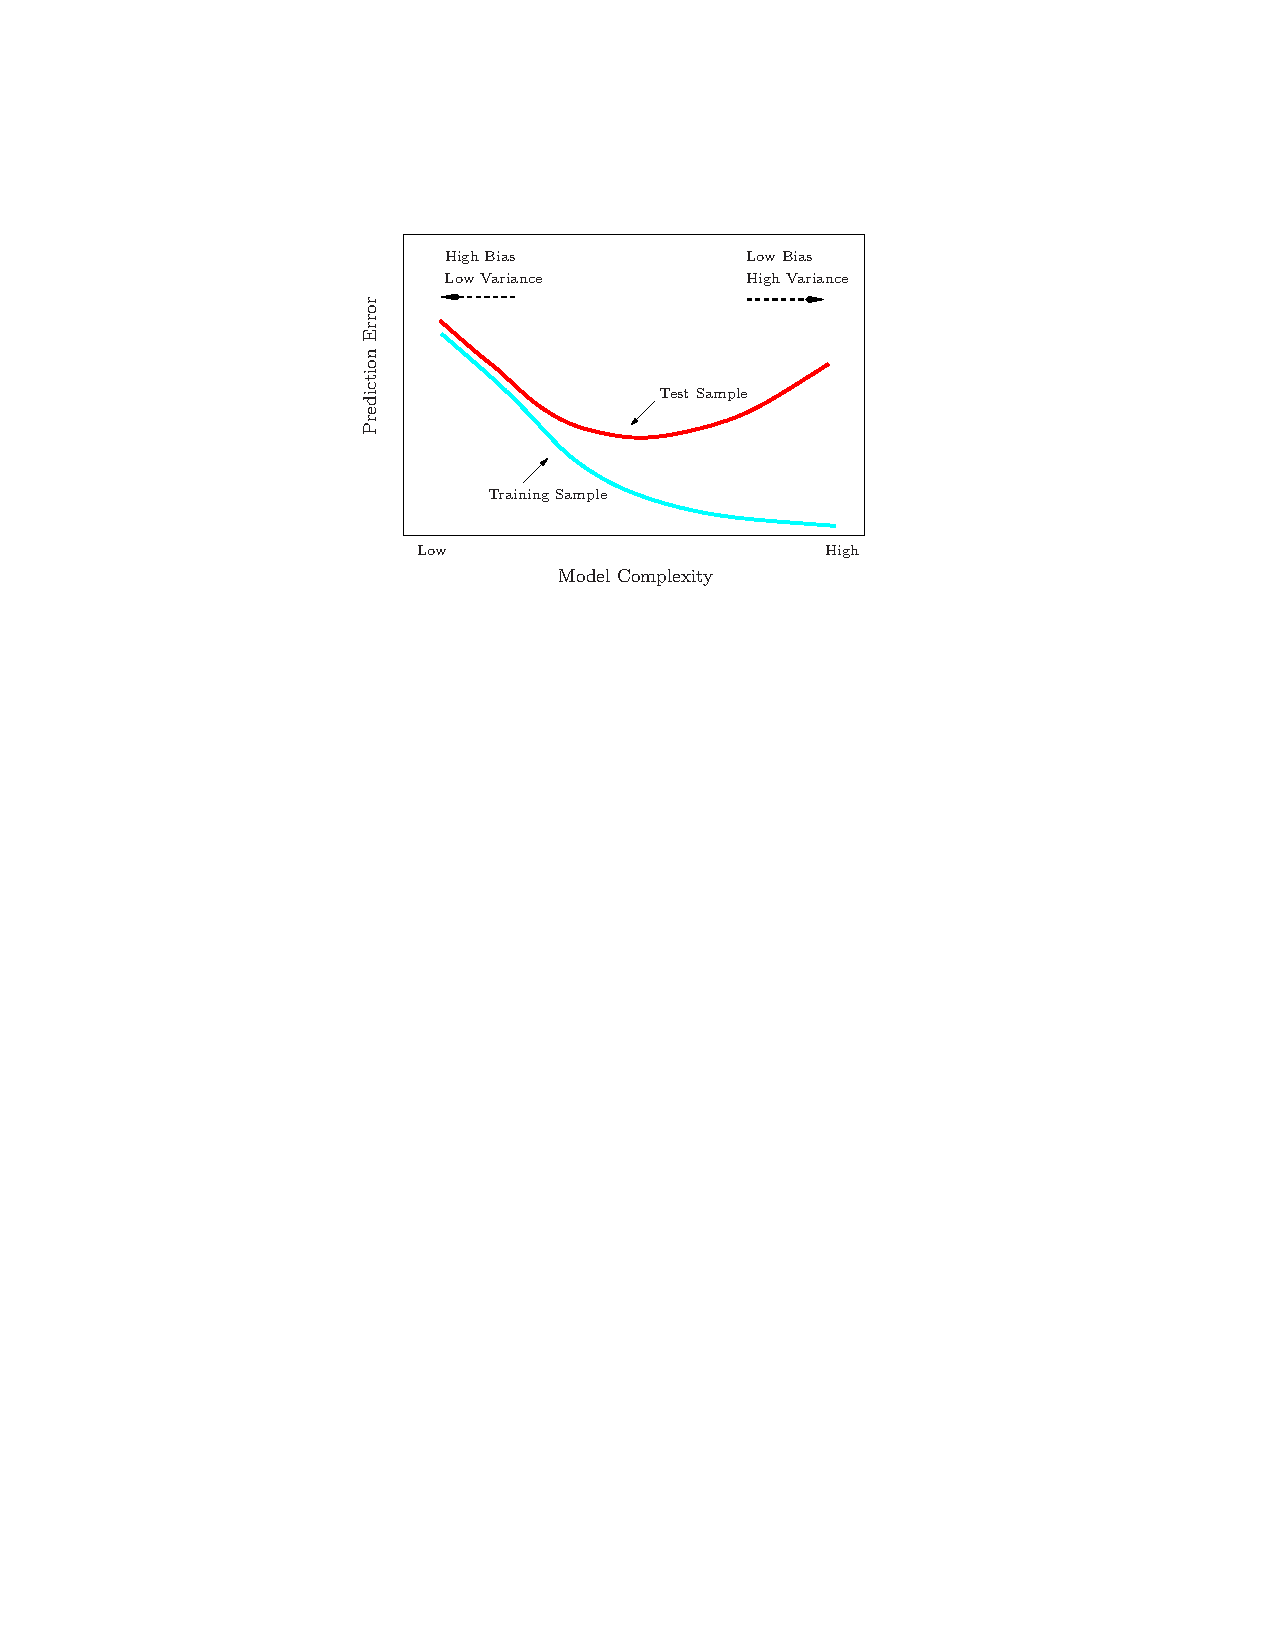
\includegraphics[width=4.5in]{ESL_bias_variance.pdf}
  \caption{The general phenomenon of Bias-Variance tradeoff over model
  complexity. Source: ESL}
\end{figure}
~\\
For example, here are bias-variance tradeoffs in classification (here the error
  is not simply the sum of bias squared and variance, but the phenomenon is
  still evident:
  Here are two other examples of the bias-variance decomposition for square loss - 
\begin{figure}[H]
  \centering
  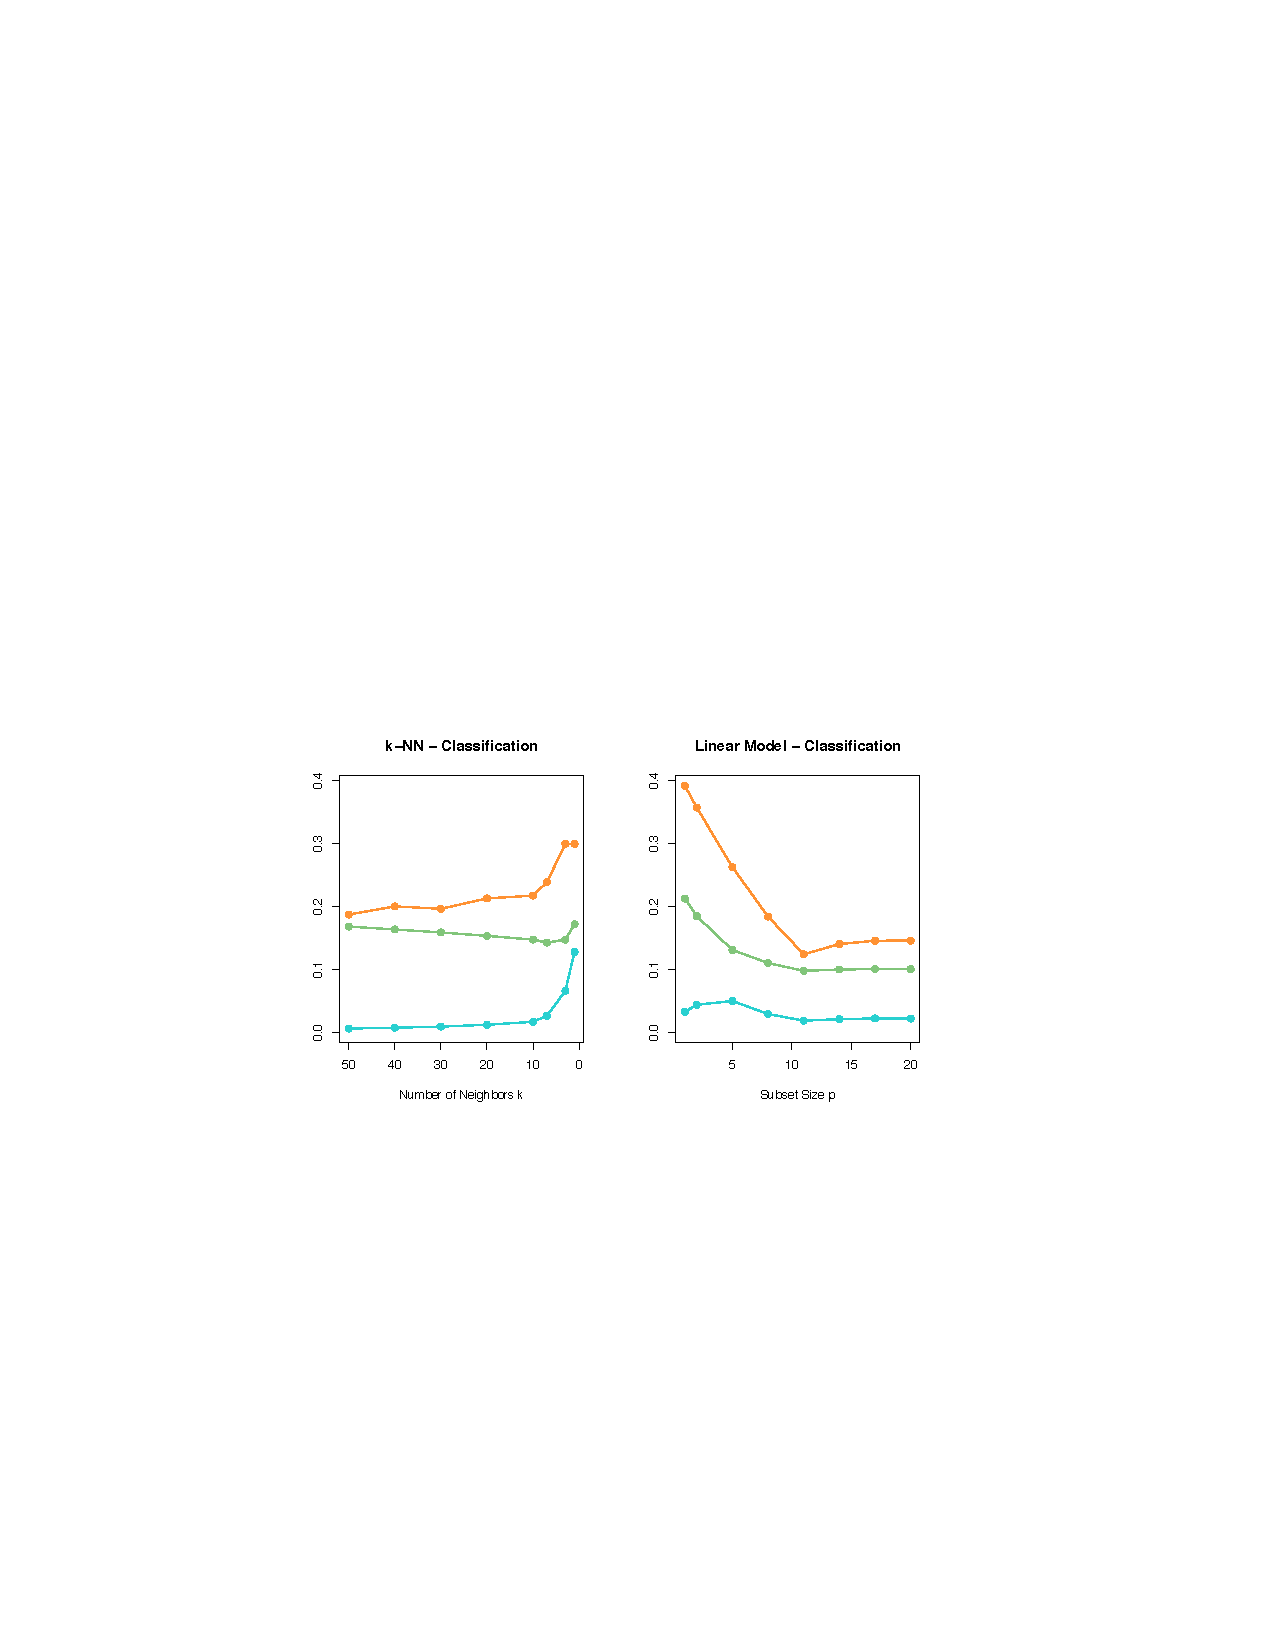
\includegraphics[width=4.5in]{esl_bias_variance_classification.pdf}
  \caption{Bias-Variance tradeoff in simulation. Left: $k$-NN classification. Right:
    Classification using Best-subset regression. Horizontal axis - left: $k$ the number of nearest
    neighbors, right: $p$ the subset size. Orange - generalization error, green
    - square bias, blue - variance.
  Source: ESL}
\end{figure}

~\\
So when we have control over the model complexity (which is usually the case),
the challenge of model selection is to locate the ``sweet-spot'' where the bias
and the variance are not too high - the point where we get the lowest
generalization error.
\\~\\
But how do we do that?



\section{Can't naively use training sample for model selection / evaluation}

We are in supervised batch learning setting. This means we have a training
sample $S$. The most naive approach for model selection and evaluation is simply
to use $S$ for everything. This would look something like that. Given a family
of learning algorithms $\{\Ac_\alpha\}$, do the following:
\begin{itemize}
  \item {\bf (Training stage.)} Train each of them on $S$ and obtain $h_\alpha=\Ac_\alpha(S)$
  \item {\bf (Model selection stage.)} Choose the best one using 
    \[
      \alpha^* := \text{argmin}_\alpha L_S(h_\alpha)
    \]
  \item {\bf (Model evaluation stage.)} 
    Estimate the generalization error of the chosen trained model $h_{\alpha^*}$
    by
    its empirical risk on $S$, namely estimate $L_\Dc(h_{\alpha^*})$ by
    $L_S(h_{\alpha^*})$
    
\end{itemize}
~\\
As we know already, {\bf this will fail miserably}: the model we select $\alpha^*$
will not have the best generalization, and the estimate 
$L_S(h_{\alpha^*})$ will be very optimistic for the actual generalization error
we will observe. (In fact {\bf optimism} is the technical term for the difference
between the empirical risk and the generalization error.)
\\~\\
Why? The learner tries to adapt as much as possible (within the choice of
$h\in\Hc$ allowed to it) to the training data. The more variance the learner
has, the more it will adapt to particular properties of the training sample $S$.
\\~\\
The following figure shows this general phenomenon.

\begin{figure}[H]
  \centering
  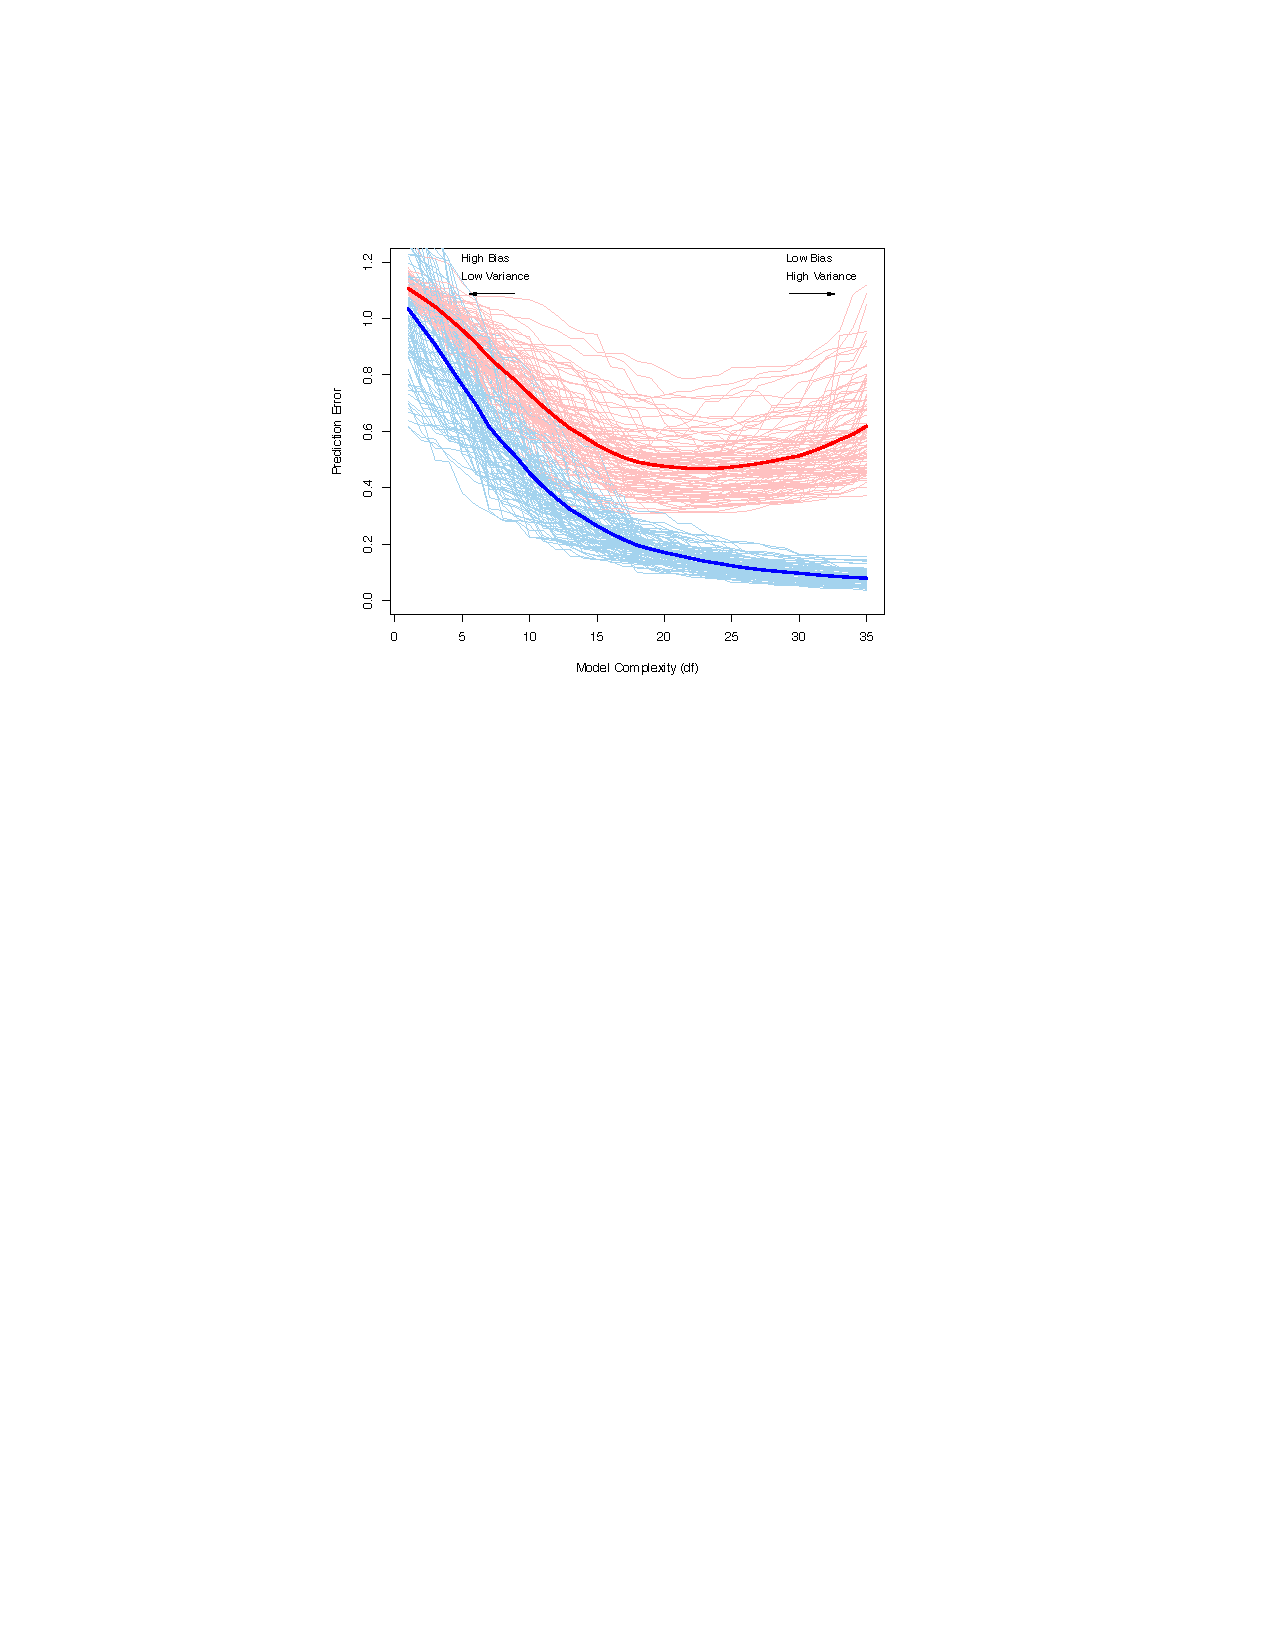
\includegraphics[width=4in]{train_vs_gen.pdf}
  \caption{Train error and generalization error over model complexity. Blue is
    training error (empirical risk), Red is generalization error. Each thin line
    is a different random sample of training sample (blue) and test sample
    (red).  Source: ESL}
\end{figure}

\section{Model selection and evaluation with unlimited data}

So using $S$ naively for everything won't work.
Let's go to the other extreme for a moment: 
If we had unlimited data, how would we approach model selection and model
evaluation? We would use three different data sets 
for the three tasks of training, model selection and model evaluation. 
Suppose we have three such samples $S$ (training), $V$ (validation), $T$ (test). 
We would do the following:
\begin{itemize}
  \item {\bf (Training stage.)} Train each of the models on $S$ and obtain $h_\alpha=\Ac_\alpha(S)$
  \item {\bf (Model selection stage.)} Choose the best model using 
    \[
      \alpha^* := \text{argmin}_\alpha L_V(h_\alpha)
    \]
    namely the average loss on the validation set $V$.
  \item {\bf (Model evaluation stage.)} 
    Estimate the generalization error of the chosen trained model $h_{\alpha^*}$
    by
    its empirical risk on $T$, namely estimate $L_\Dc(h_{\alpha^*})$ by
    $L_T(h_{\alpha^*})$
    
\end{itemize}

However, in batch learning we are just given our one training sample $S$. 
If we split $S$ into a smaller training sample $\tilde{S}$, a validation set $V$
and a test set $T$, we will be working with much smaller sample sizes.
\\~\\
So what can we do? Is there a way to use $S$ somehow and still do proper model
selection and evaluation? We've already seen such magic in the Bagging lecture,
where we used our one training sample $S$ as if we had a much larger dataset!
We'll do the same here.

\section{$k$-fold Cross Validation}

The idea of cross-validation is very simple. Imagine we left out a $1/5$ (say)
of the training sample $S$ as a held-out set, and trained the model on the
remaining $4/5$. For a candidate model $h$, we use the held-out set (that $1/5$
of $S$ that we left out) to calculate the prediction error. But hey, why not
repeat this same trick five times, each time leaving a different chunk out and
training on the rest?
\\~\\
In $k$-fold Cross Validation we divide the training set $S$ into $k$ equal
parts, at random. 

\begin{center}
  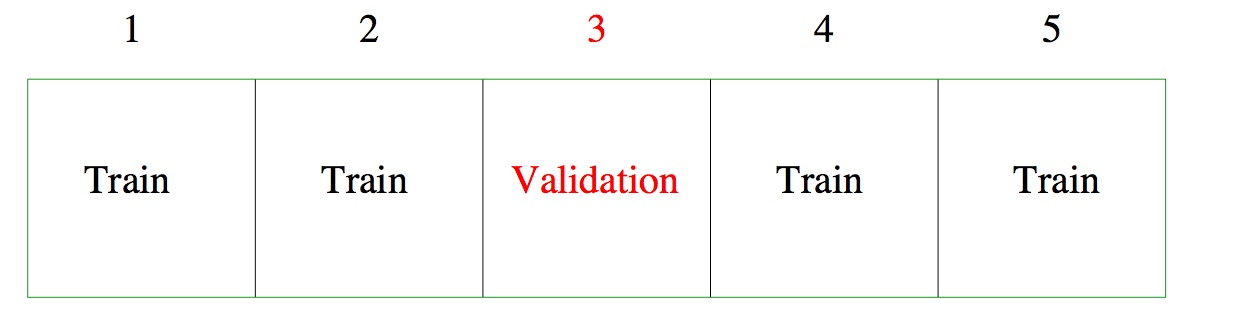
\includegraphics[width=4in]{cv.jpeg}  
    \end{center}
    \begin{itemize}
      \item We then proceed as follows. For $i=1\cdots k$:
      \begin{itemize}
        \item Train the $i$-th model on all the data {\bf except} the $i$-th fold
        \item Calculate the loss of the trained $i$-th model on the $i$-th fold, acting as a test set
      \end{itemize}
    \item Report the estimated mean and standard deviation of the $k$ losses obtained.
  \end{itemize}
~\\
  (Do you remember how to estimate standard deviation?)


  \subsection{Cross validation for model selection}
  Cross validation is the most popular method for choosing tuning parameters.
  To do this, we train each of the candidate learners $\Ac_\alpha$ $k$ times -
  each time leaving out one of the $k$ folds. (So you see this can be pretty
  computationally intensive.) We then choose the learner $\Ac_\alpha$ whose
  average error (over the $k$ test sets) was lowest.
\\~\\
  Many software packages (e.g. for regularized learners) offer implementation of cross
  validation for choosing the regularization parameters.

  
  \begin{figure}[H]
    \centering
  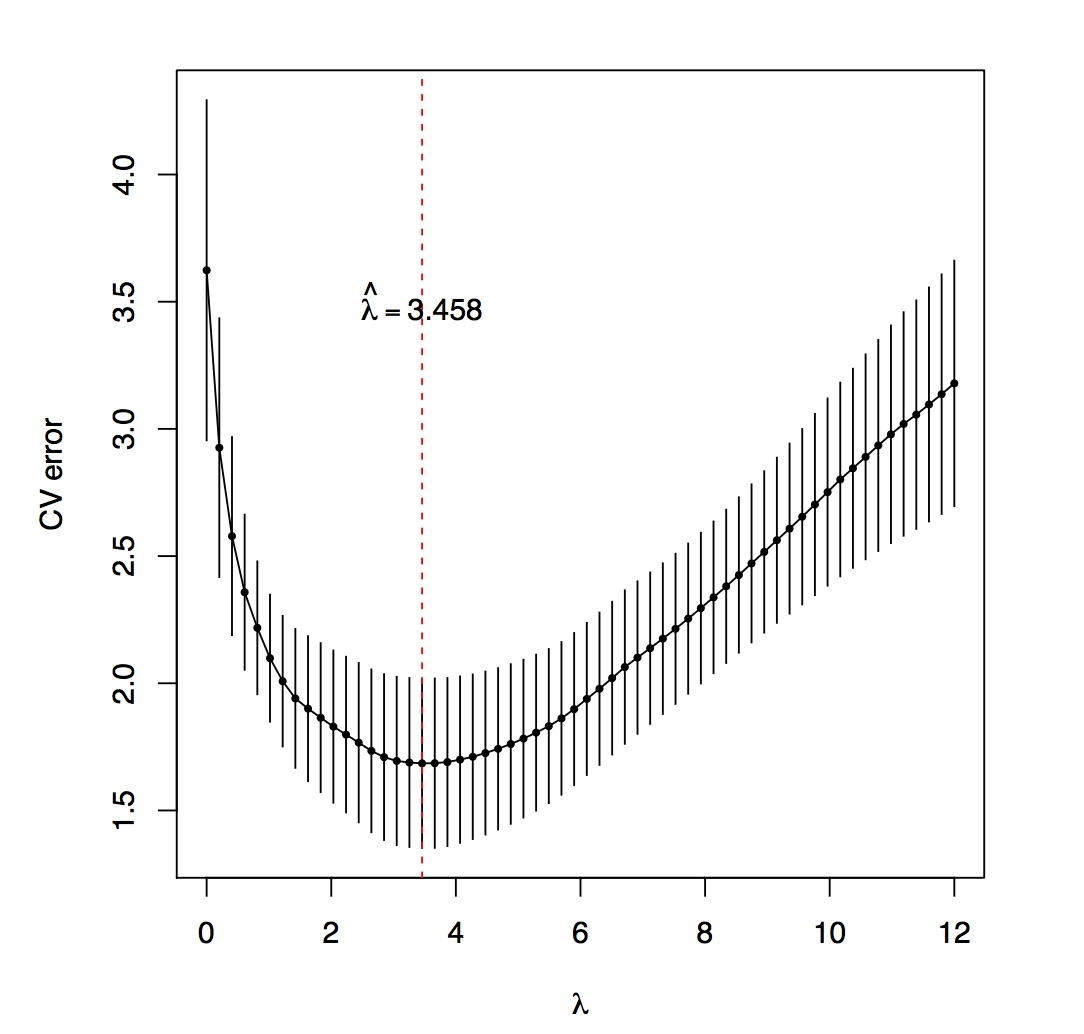
\includegraphics[width=4in]{cv_lambda.jpeg}  
      \caption{Plot produced by the package {\tt glmnet} for choosing $\lambda$
      for regularized regression by cross validation}
  \end{figure}

  {\bf Important note.} After we finish model selection with cross validation,
  and have a fully specified learner $\Ac$, we train $\Ac$ {\bf again} on the
  entire training sample $S$. We would like to train $\Ac$ on as many points as
  possible, so for the actual prediction we do not use any of the models trained
  on parts of $S$.

  \subsection{Cross validation for model evaluation}
  Cross validation is also used for model evaluation. Once we have a final,
  fully specified learner $\Ac$, we run $k$-fold cross validation and report
  both the average error over the $k$ folds, and its standard deviation. So we
  estimate the generalization loss and also provide some measure of accuracy
  of this estimate. 
\\~\\
Does it work? Here is a simulation experiment comparing the true generalization
loss to the estimate obtained by 10-fold cross validation:
\begin{figure}[H]
  \centering
        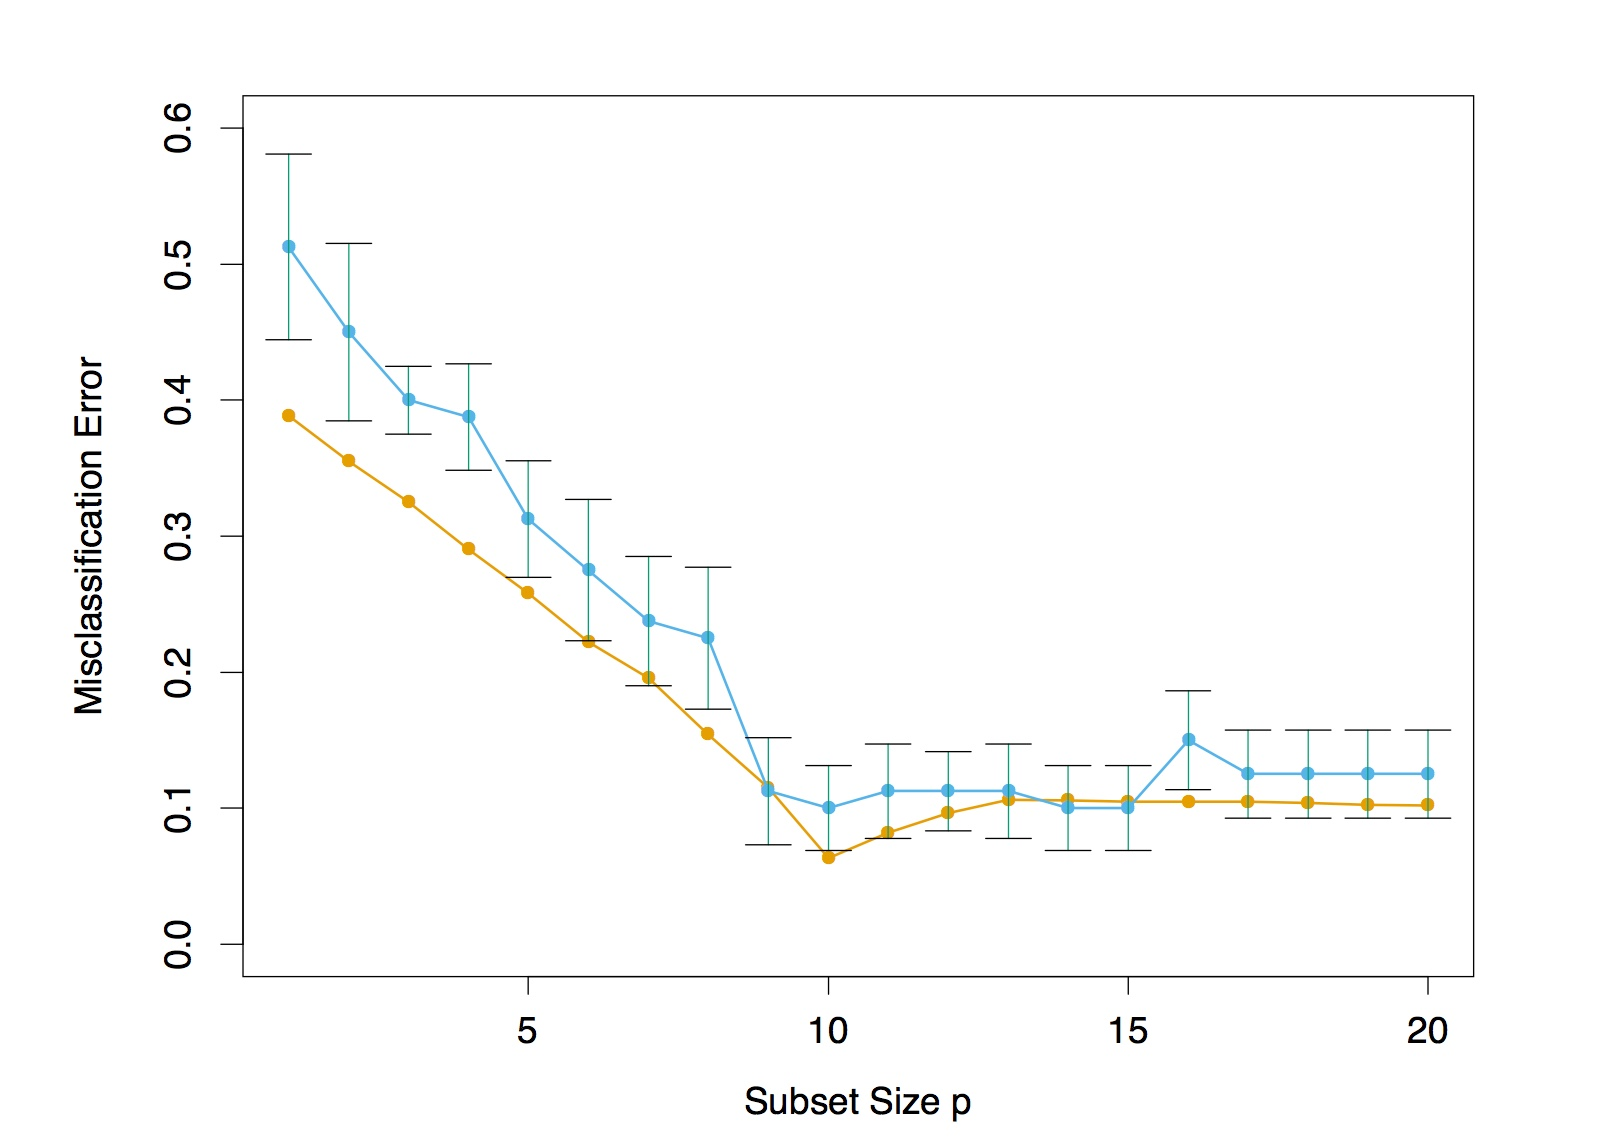
\includegraphics[width=4in]{cv_vs_test.jpeg}  
      \caption{
      Generalization error (orange) and 
      10-fold cross-validation error (with errorbars,
    blue) over model complexity for some learning problem. Source: ESL}
\end{figure}



    \subsection{Considerations in choosing number of folds $k$}
      \begin{itemize}
    \item If $k=1$ then no CV
\item If $k=2$ (``split-sample CV'') we only train on half the data, so CV error
  will be larger than true out-of-sample error
\item Small $k$ - we may be training on a dataset too small so again CV error
  may be {\bf biased upwards}
\item Large $k$ - All training sets are almost the same, so we're in CV errors
  we're averaging
  highly correlated random variables. May introduce high variance 
    \item if $k=m$ (sample size) this is {\bf leave-one-out} CV
    \item Since we train the model $k$ times, large $k$ can be computationally
      intensive
  \end{itemize}
 



\section{Bootstrap}

Recall the bootstrap - the basis for the Bagging meta-algorithm. 
\\~\\
The Bootstrap can also be used for estimating generalization error - for model
selection or evaluation - based on just the one training sample $S$ that we
have. 
\\~\\
To estimate generalization error of a learner $\Ac$, we draw B bootstrap samples
(each bootstrap sample has $m$ resamples from $S$ with replacements). 
Call the $b$-th Bootstrap sample $S^{(b)}$. 
Define the $b$-th test set by 
$T^{(b)}:= S\setminus S^{(b)}$ - namely, all the points of $S$ that were {\bf
not} chosen in the $b$-th bootstrap sample. 
 (The samples that were not included are called {\bf
out-of-bag} samples.)
Now train $\Ac$ on $S^{(b)}$ and
test it on $T^{(b)}$.
 Report the estimated mean and standard deviation of the
generalization errors, as measured on the $B$ test sets. 

\section{Two common mistakes in model evaluation and how to avoid them}

There are two very common mistakes when using cross validation or bootstrap for
model evaluation. 
One mistake causes us to over-estimate the generalization error (so our estimate
is too high, too pessimistic). The other causes us to under-estimate the
generalization error (so our estimate is too low, too optimistic).

\subsection{Over-estimating generalization error}

Take for example cross validation, used for model evaluation of a fully
specified learner $\Ac$. In cross validation, we train $\Ac$ on a training set
smaller than $S$ - in fact we train it on $m(k-1)/k$ where $|S|=m$ and $k$ is
the number of folds we use in our cross-validation. If $k$ is not large, this
means that each time we train during cross validation, we reduce the number of
available samples. 
\\~\\
Recall from PAC theory (for example) that there is a minimal number of samples
needed to learn an hypothesis from a given hypothesis class. What if $|S|=m$ is
enough, but $m(k-1)/k$ is not enough? In this case the cross-validation estimate
will over-estimate the generalization error. 
\\~\\
We realize that it's a good idea to know how the number of training samples
affects the learning algorithm we are studying. For every learner there is
a curve describing generalization error as a function of training sample size
$m$. If we can somehow estimate this curve, we can be smarter about choosing the
number of folds $k$ given the training sample size $m$ that we have.
      
\begin{figure}[H]
  \centering
  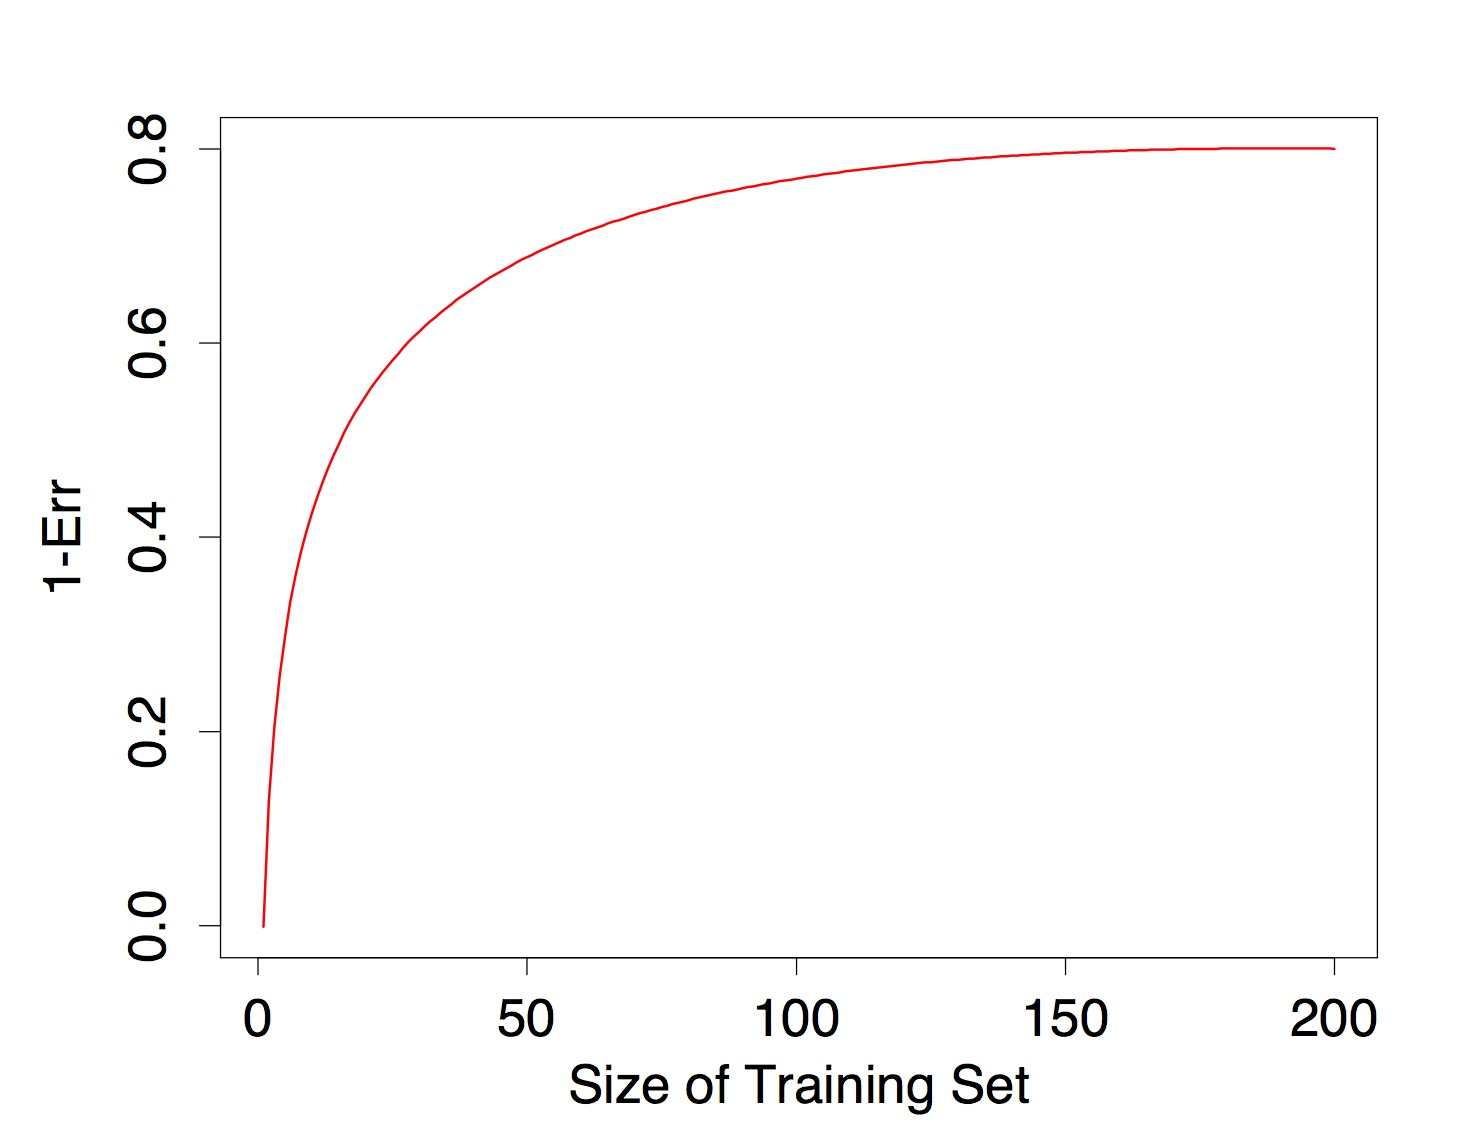
\includegraphics[width=3.3in]{learning_curve.jpeg}  
  \caption{{\bf Exercise}: Suppose this is the generalization error of a learner
    $\Ac$ as function of training sample size. We would like to estimate
    generalization error of $\Ac$ using $k$-fold cross validation. 
    Suppose our data has $m=200$ samples.  Will 5-fold CV give a good estimator
of out-of-sample error? Now
suppose $m=50$. Has anything changed? Source: ESL }
\end{figure}



\subsection{Under-estimating generalization error}

A much more common problem is that cross-validation estimates for generalization
error are too optimistic. This is a subtle yet very important point for you to
understand.  
\\~\\
The following is a very common process:
\begin{itemize}
      \item Suppose we have a dataset with $m$ samples and cannot get more data
      \item We start trying out models, each with its own tuning parameters.
        This can be called {\bf model snooping}
      \item We change the training sample $S$ - remove features, create new
        features, 
        remove ``problematic'' points, etc. This can be called {\bf data
        snooping.} 
      \item Eventually we find a tuned model and a ``clean training sample'' that ``work well'' \ldots
      \item \ldots namely has low training error, fits the data well, etc
      \item {\bf Now} we use cross validation or bootstrap to estimate the
        generalization error of our chosen learner.
    \end{itemize}

    What's the problem? 
\\~\\
    There are two problems here:
    \begin{itemize}
      \item 
    One, the problem with model snooping. By obsessively tuning and tuning and trying out many learners, we overfit to
    the training sample. And if we use a validation set, after using it many
    many times, we overfit to the validation set as well.
  \item
    Two, the problem with data snooping. When new, unseen data comes in, it did not receive this
    royal treatment we gave to the training sample $S$. So the cross validation
    procedure under-estimates performance on new data.

\end{itemize}

~\\   
You should be familiar with the {\bf mechanism of self-deception} 
in machine-learning. It works as follows:
    \begin{itemize}
      \item You start working on a dataset and really want ``good results''
      \item You try many methods, many tuning parameters
      \item You make some changes in the training sample $S$ 
      \item Gradually as you overfit you sink into self-deception
      \item This is called ``Torture the data until they confess''
    \end{itemize}


\subsection{What can we do to avoid under-estimating generalization error?}

\begin{enumerate}
  \item Avoid manual data snooping. {\bf Code the entire pre-processing stage}.
    At each iteration of Bootstrap or cross-validation, run the entire
    pre-processing step - just like it would run when you predict on new data.
  \item Limit model snooping and data snooping to a small subset of $S$ which
    you know will be ``contaminated with optimism''. If keeping a held-out set
    for use in a later stage of the learner design, lock it and guard the key
    with your life. Remember you will be tempted to peek at this set, and
    resist. 
\end{enumerate}


\end{document}

%
%
%
%N = length(X); % X training labels
%    W = 1/N * ones(N,1); %Weights initialization
%    M = 10; % Number of boosting iterations 
%
%    for m=1:M
%        C = 10; %The cost parameters of the linear SVM, you can...
%                 perform a grid search for the optimal value as well           
%
%        %Calculate the error and alpha in adaBoost with cross validation
%        cmd = ['-c ', num2str(C), ' -w ', num2str(W)];
%        model = svmtrain(X, Y, cmd);
%        [Xout, acc, ~] = svmpredict(X,Y,cmd);
%
%        err = sum(.5 * W .* acc * N)/sum(W);
%        alpha = log( (1-err)/err );
%
%        % update the weight
%        W = W.*exp( - alpha.*Xout.*X );
%        W = W/norm(W);
%
%    end
